\documentclass[a4paper]{article}
\usepackage[utf8]{inputenc}
\usepackage{fancyhdr}
\usepackage{vmargin}
\usepackage{listings}

%nicer tables
\usepackage{booktabs}

\usepackage{graphicx}

\usepackage{float}

\usepackage{color}
\usepackage{url}
\usepackage{hyperref}

\usepackage{enumerate}

\usepackage[backend=biber]{biblatex}

\usepackage{csquotes}

\usepackage{multicol}
\setlength{\columnsep}{1cm}
\setlength{\headheight}{36pt}

\definecolor{bluekeywords}{rgb}{0.13,0.13,1}
\definecolor{greencomments}{rgb}{0,0.5,0}
\definecolor{redstrings}{rgb}{0.9,0,0}



%
\usepackage{amsmath, amsthm, amssymb}
\usepackage[ngerman, english]{babel}
\usepackage{marvosym}
\usepackage{graphics}
\usepackage{extarrows}
\usepackage{forloop}
\usepackage{mathtools}

\usepackage[]{algorithm2e}

\usepackage{hyperref}% http://ctan.org/pkg/hyperref
\usepackage{cleveref}% http://ctan.org/pkg/cleveref
\usepackage{lipsum}% http://ctan.org/pkg/lipsum
\newtheorem{definition}{Definition}
\newtheorem{theorem}{Theorem}
\newtheorem{lemma}{Lemma}
\newtheorem{preliminary}{Preliminary}
\newtheorem{notation}{Notation}
\newtheorem{property}{Property}
\newtheorem{corollary}{Corollary}
\newtheorem{example}{Example}
\newtheorem{hypothesis}{Hypothesis}

\crefname{theorem}{Theorem}{Theorems}
\crefname{definition}{Definition}{Definitions}
\crefname{lemma}{Lemma}{Lemmas}
\crefname{preliminary}{Preliminary}{Preliminaries}
\crefname{notation}{Notation}{Notations}
\crefname{property}{Property}{Properties}
\crefname{corollary}{Corollary}{Corollaries}
\crefname{example}{Example}{Examples}
\crefname{hypothesis}{Hypothesis}{Hypotheses}

\newenvironment{beweis}{\begin{proof}[Beweis]}{\end{proof}}
%



\lstset{language=Python,
showspaces=false,
showtabs=false,
breaklines=true,
showstringspaces=false,
breakatwhitespace=true,
escapeinside={(*@}{@*)},
commentstyle=\color{greencomments},
keywordstyle=\color{bluekeywords}\bfseries,
stringstyle=\color{redstrings},
basicstyle=\ttfamily
}


\setlength{\parindent}{0pt}
\setlength{\parskip}{5pt}

\frenchspacing
\pagestyle{fancy}
\sloppy 

\markright{headline}

\addbibresource{references.bib}

\begin{document}

\lhead{\begin{tabular}{l}
\\
Neural Networks\\
WiSe 2020/2021\\
\end{tabular}}

\rhead{\begin{tabular}{r}
Assignment 6\\
Simon Laurent Lebailly, 2549365, s9sileba@teams.uni-saarland.de\\%% <=== Also HERE if you have a team mateUpdate Name HERE !!! 
Christian Mathieu Schmidt, 2537621, s9cmscmi@teams.uni-saarland.de
\end{tabular}}




\section*{Exercise 7.1: $L_1$ and $L_2$ Regularization}
    \subsection*{a)}
        \begin{center}
            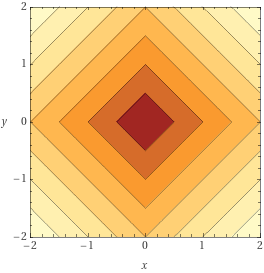
\includegraphics[width=55mm]{Assignment 7/L1(2).png}
            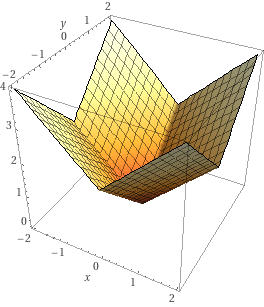
\includegraphics[width=55mm]{Assignment 7/L1(1).png}\\
            \caption{$L_1$ Contour-plot and 3D-plot (plotted at https://www.wolframalpha.com)}
        \end{center}
        \begin{center}
            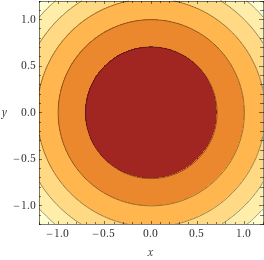
\includegraphics[width=55mm]{Assignment 7/L2(2).png}
            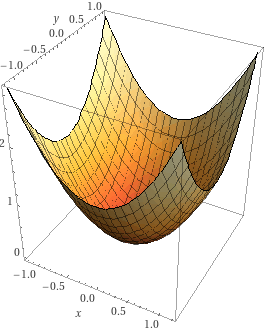
\includegraphics[width=55mm]{Assignment 7/L2(1).png}\\
            \caption{$L_2$ Contour-plot and 3D-plot (plotted at https://www.wolframalpha.com)}
        \end{center}


    \subsection*{b)}
        $L_1$ produces a spase model, because most of its parameters will become equal to zero, provided the hyperparameter is large enough.
        So $L_1$ performs feature selection by deciding which features are essential for prediction and which are not.
        So $L_1$ is prefered, if we want to increase the model explainability.

    
    \subsection*{c)}
        Yes it is possible and is called "elastic net regularization", which has $L_1$ and $L_2$ regularizations as special cases.
        Elastic net regularization linearly combines the L1 and L2 penalties of the lasso and ridge methods and can be reduced to the linear support vector machine.\footnote{https://www.aaai.org/ocs/index.php/AAAI/AAAI15/paper/view/9856}
        The reduction immediately enables the use of highly optimized SVM solvers for elastic net problems. It also enables the use of GPU acceleration, which is often already used for large-scale SVM solvers.\footnote{https://ttic.uchicago.edu/~cotter/projects/gtsvm/}
    
    \subsection*{d)}
        Regularization encompasses methods that force the learning algorithm to build a less complex model.
        In practice, that often leads to slightly higher bias but reduces the variance significantly (bias-variance tradeoff).
        The idea of regularization is to modify the objective function by adding a penalizing term whose value is higher when the model is more complex.
        So, regularization decreases the generalization error by increasing, or in better words not reducing, the training error.
        This is only important if there is a risk to overfit the model. 

    
    \subsection*{e)}
        \begin{center}
            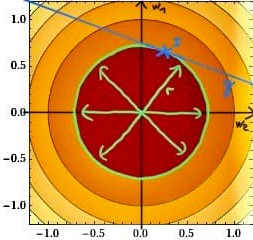
\includegraphics[width=80mm]{Assignment 7/L2(3).jpg}\\
            \caption{$L_2$ Contour-plot for an example (plotted at https://www.wolframalpha.com)}
        \end{center}
        Let us consider the contours of the plot as different growth layers of the circle.
        As you can see on the plot, the straight line $g$ intersects the green circle growing from the center in the direction of the green arrows at exactly one point, which is the minimum of the $L_2$ regularization. 
        This intersection point s has the coordinates $(w_1|w_2)$ with $w_1,w_2 < r$ (where $r$ is the radius of the green circle).
        So $w_1$ or $w_2$ become zero only if the straight line would intersect one of the main axes at the point $r$.
        In this case $g$ would be parallel to the $w_1$ or $w_2$ axis.
        Assuming that $g$ intersects the $w_2$ axis at point $r$, the other case is analogous.
        Mathematically this would mean that $w_2 = r$ and $w_1=0$, where $w_1$ would play no role at all for the consideration of the original problem.
        But since this case cannot occur, that $g$ is parallel to a major axis, since $w_2$ is a weight which varies, no variable can be set equal to zero by $L_2$!
        Here I have taken two weights as an example, but the same is true for any number of weights, if one weight would intersect an axis at the point $r$.\\
        More mathematical, for $n$ weights we have to solve the problem:
        \begin{align}
            w_1 + ... + w_n &= a\\
            \text{and}\ \ \ \min_{w_1,...,w_n}\{w^2_1 + ... + w^2_n\} &= a
        \end{align}\ \\

    \subsection*{f)}
        \begin{center}
            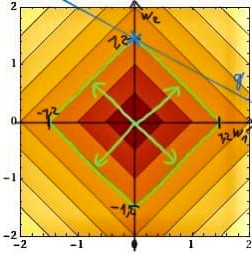
\includegraphics[width=80mm]{Assignment 7/L1(3).jpg}\\
            \caption{$L_1$ Contour-plot for an example (plotted at https://www.wolframalpha.com)}
        \end{center}
        Let us consider the contours of the plot as different growth layers of the lasso-diamond.
        As you can see on the plot, the straight line $g$ intersects the green lasso-diamond growing from the center in the direction of the green arrows at exactly one point, which represents the minimum of the $L_1$ regularization. 
        This intersection point s has the coordinates $(0|w_2)$.
        So there are exactly three possibilities how the lasso-diamond can intersect a straight line.
        Either it touches the line at a point, or, if the line is parallel to the edge of a lasso-diamond, all points on this lasso edge are a solution for the minimization problem.
        If the solution has to be only one intersection point, the lasso-diamond has to intersect the straight line along one of the principal axes.
        From this follows that at least one weight must be zero!
        Here I have taken two weights as an example, but the same is true for any number of weights, if at least one weight intersects a principal axis.\\
        More mathematical, for $n$ weights we have to solve the problem:
        \begin{align}
            w_1 + ... + w_n &= a\\
            \text{and}\ \ \ \min_{w_1,...,w_n}\{|w_1| + ... + |w_n|\} &= a
        \end{align}


\newpage
\section*{Exercise 7.2: Multi-Task Learning and Data Augmentation}
    \subsection*{a)}
        \begin{enumerate}
            \item \textbf{Problem 1:}
                    
                \textbf{Solution1:}
        \end{enumerate}
    
    \subsection*{b)}



\newpage
\section*{Exercise 7.3: Early Stopping}
    \subsection*{a)}
        Under the assumption (i) $|1-\epsilon\lambda_j| < 1$, it holds that
        \begin{align}
            \lim_{\tau \rightarrow \infty} \omega^{\tau}_j &= \lim_{\tau \rightarrow \infty} \{1 - (\underbrace{1 - \epsilon\lambda_j}_{< 1\ (i)})^{\tau}\} \omega^{*}_j\\
            &= \{1 - 0\} \omega^{*}_j = \omega^{*}_j
        \end{align}
        $\Rightarrow$ If the number of steps $\tau$ goes to infinity, then each component of the weight vector $\omega^{\tau}_j$ converges to the corresponding component $\omega^*_j$ of the minimum! Thus it is valid for the weight vector $\omega$ that 
        \begin{align}
            \lim_{\tau \rightarrow \infty} \omega^{\tau} &= \omega^*
        \end{align}
    
    \subsection*{b)}
        \begin{itemize}
            \item \textbf{To show:} $\omega^{\tau}_j \simeq \omega^*_j$ when $\lambda_j \gg (\epsilon\tau)^{-1}$
            \begin{proof}
                If $\lambda_j \gg (\epsilon\tau)^{-1}$ then we know that
                    \begin{align}
                        1-\epsilon\lambda_j \ll 1-\frac{\epsilon}{\epsilon\tau} = 1-\frac{1}{\tau} = \frac{\tau-1}{\tau}
                    \end{align}
                Because $\tau > 0$ we can follow
                    \begin{align}
                        \left(\frac{\tau-1}{\tau}\right)^{\tau} = \frac{(\tau-1)^{\tau}}{\tau^{\tau}} \ll 1
                    \end{align}
                Thus we can follow that
                    \begin{align}
                        1-(1-\epsilon\lambda_j)^{\tau} \simeq 1-0 = 1
                    \end{align}
                And so we can conclude that
                    \begin{align}
                        \omega^{\tau}_j = \{1 - (1 - \epsilon\lambda_j)^{\tau}\} \omega^{*}_j 
                        \simeq \{1\} \omega^{*}_j = \omega^*_j
                    \end{align}
            \end{proof}
            
        \end{itemize}
    
    \subsection*{c)}



\newpage
\section*{Exercise 7.4: Universal Approximation Theorem}
    \subsection*{a)}
        The main idea of the paper "concisely cited" best describes this parts of the abstract:
        \begin{quote}
            \textit{"... standard multilayer feedforward networks with as few as a single hidden layer and arbitrary bounded and nonconstant activation function are universal approximators with respect to $L^P(\mu)$ performance criteria ..."}
        \end{quote}
        \begin{quote}
            \textit{"We also give very general conditions ensuring that networks with sufficiently smooth activation functions are capable of arbitrarily accurate approximation to a function and its derivatives."}
        \end{quote}
        And this part of the concluding remark:
        \begin{quote}
            \textit{"...multilaver feedforward networks are, under very general conditions on the hidden unit activation function, universal approximators, provided that sufficiently many hidden units are available..."}
        \end{quote}
        In simple words, the paper shows, that multilayer feedworward networks can approximate every algorithmically generated function (universal approximation theorem).
    
    \subsection*{b)}
    In this paper the authors only consider finite linear combinations of compositions of fixed, univariate functions with support in the unit hypercube, with an arbitrary continuous sigmoidal nonlinearity, restricted only to single hidden layer neural networks.
    Thus the main difference are the number of the hidden layers of the considered neural networks.
    So the paper in Part a considers general conditions on multilayer networks, and this paper only considers univariate functions on single hidden layer neural networks.
    This is only a special case of the paper in Part a, which shows, that multilayer feedworward networks can approximate every algorithmically generated function.
    Thus the result in this paper is weaker than the paper in Part a.\\\\
    The main idea of the paper best describes this part of the summary:
    \begin{quote}
        \textit{"We have demonstrated that finite superpositions of a fixed, univariate function that is discriminatory can uniformly approximate any continuous function of $n$ real variables with support in the unit hypercube. Continuous sigmoidal functions of the type commonly used in real-valued neural network theory are discriminatory.
        This combination of results demonstrates that any continuous function can be uniformly approximated by a continuous neural network having only one internal, hidden layer and with an arbitrary continuous sigmoidal nonlinearity."}
    \end{quote}
    
    \subsection*{c)}
        The hierarchical structure of deep networks makes them particularly useful to learn the hierarchies of knowledge, for example problems like image recognition. 
        In such cases, a system that understands not just individual pixels, but also more complex concepts, from edges to simple geometric shapes, all the way up through complex, multi-object scenes, can be very useful!
        Such an "overview" on upbuilding structures is not realizable for neural networks with few hidden layers.

\end{document}
